\section{Experimentación}
%Merge de las secciones Resultados y Discusion
%Experimentación:
%Deben incluir los resultados de los experimentos, utilizando el formato m´as adecuado
%para su presentaci´on. Deber´an especificar claramente a qu´e experiencia corresponde
%cada resultado. No se incluir´an aqu´ı corridas de m´aquina.
%Discusión:
%Se incluir´a aqu´ı un an´alisis de los resultados obtenidos en la secci´on anterior (se analizar´a
%su validez, coherencia, etc.). Deben analizarse como m´ınimo los ´ıtems pedidos en el
%enunciado. No es aceptable decir que “los resultados fueron los esperados”, sin hacer
%clara referencia a la teor´ıa a la cual se ajustan. Adem´as, se deben mencionar los resultados
%interesantes y los casos “patol´ogicos” encontrados.
En esta sección estudiaremos, mediante experimentaciones,
como varía la calidad de los resultados obtenidos al cambiar el parámetro\textit{ k }de kNN.
También observaremos qué sucede al cambiar la frecuencia mínima y máxima de palabras a filtrar
y cómo afecta el tamaño del dataset.
Cuando usamos PCA, queremos ver cómo impacta modificar el valor de alpha
y la cantidad de veces que ejecutamos el Método de la Potencia en la calidad de los resultados.
En todos los casos, la calidad de los resultados de clasificación obtenidos
será analizada mediante su \textit{accuracy}, el cual es definido como

\begin{itemize}
	\item $ \textit{Accuracy} = \frac{Verdaderos Positivos + Verdaderos Negativos}{Cantidad Total de Predicciones} $
\end{itemize}

Además, queremos experimentar sobre cómo afecta al tiempo de ejecución del programa usar o no PCA,
y cómo se ve impactado por el tamaño del training data.

\subsection{Experimentación sobre kNN}
En esta sección desarrollaremos los distintos experimentos realizados para ver
la calidad de resultados al ejecutar kNN, sin PCA previo, cambiando distintos
parámetros. Además analizaremos los tiempos de ejecución de las pruebas en la sección \ref{sec:knnvstrain}.

\subsubsection{Experimentación sobre k}
Comenzamos experimentando con la cantidad de vecinos a considerar (parámetro k)
en el algoritmo de kNN.
Queremos ver cómo varía la métrica de \textit{accuracy} a medida que crece el\textit{ k }usado.

Lo que esperamos ver es que a medida que aumentemos k, el \textit{accuracy} aumente
hasta un cierto punto y luego comience a descender.
Creemos que usando un\textit{ k }demasiado chico, puede suceder que califiquemos mal por quedar
demasiado cerca de algunos outsiders, pero al considerar muchos vecinos
dejamos de darle importancia al valor de los más cercanos.
Es decir, estaríamos calculando el promedio de cierta sección en el espacio
quitándole importancia a la posición relativa en donde se encuentra el vector a
predecir y asignandole esa polaridad, sesgando así el resultado del algoritmo hacia el valor mayoritario.

%grafico
Para probar nuestra hipótesis corrimos el programa con 6 valores de\textit{ k }y con
25000 de las 50000 reseñas como \textit{training data}. Guardamos el accuracy de cada prueba.

Queríamos hacer esta experimentación sobre\textit{ k }sin aplicar ningún filtro de frecuencias al dataset, pero dado que el tamaño de nuestro vocabulario es muy grande nos fue imposible. Correr kNN para un solo\textit{ k }habría tardado aproximadamente 16 días. Por lo tanto, decidimos aplicar el menor filtro posible que es \textbf{F}$ = 0.995$ y \textbf{f}$ = 0.001$ siendo \textbf{f} la frecuencia mínima a partir de la cual guardamos palabras y \textbf{F} la frecuencia máxima a partir de la cual borramos palabras.
Es decir, eliminamos todas las palabras que tengan menor frecuencia que \textbf{f} y mayor frecuencia que \textbf{F}.

\begin{figure}[H]
\centering
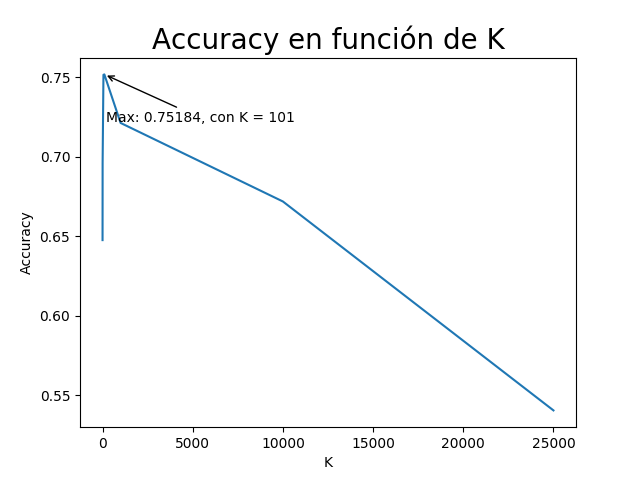
\includegraphics[ height=10cm, width=12cm]{../experimentos/graficos/graph_sin_pca_accuracy.png}
\caption{accuracy vs. valor de\textit{ k }sin PCA con F = 0.995 y f = 0.001}
\label{fig:exp_k}
\end{figure}

%conclusiones:
Luego de la experimentación, como se puede ver en la figura \ref{fig:exp_k}, verificamos nuestra hipótesis.
Observamos cómo las métricas ascienden positivamente para los primeros 101
valores de k, pero al tomar $k = 501$ las métricas comienzan a descender.

Podemos concluir mediante los resultados obtenidos que los mejores 2 valores de
k a considerar son $k = 51$ y $k = 101$, en donde 51 y 101 representan
respectivamente el 0,204\% y 0,404\% del total de valores de \textit{training}.\\

No nos quedamos conformes con el tiempo de ejecución de estas pruebas. Correr kNN para 6 valores distintos de\textit{ k }tardó aproximadamente 28 horas. Como queremos correr mucha más experimentación sobre distintas variables del programa queremos buscar una solución para poder acortar los tiempos. Lo que primero queremos ver es cómo cambian los resultados de la experimentación filtrando el vocabulario de palabras con otros valores que hagan los tiempos de ejecución más rápidos. Si no encontramos ningún filtro que cumpla con estas condiciones, vamos achicar el dataset de test ordenándolo de manera aleatoria antes.

Corrimos de vuelta el programa con los mismos parámetros cambiando solo los valores de \textbf{F}$ = 0.99$ y \textbf{f}$ = 0.01$.

\begin{figure}[H]
\centering
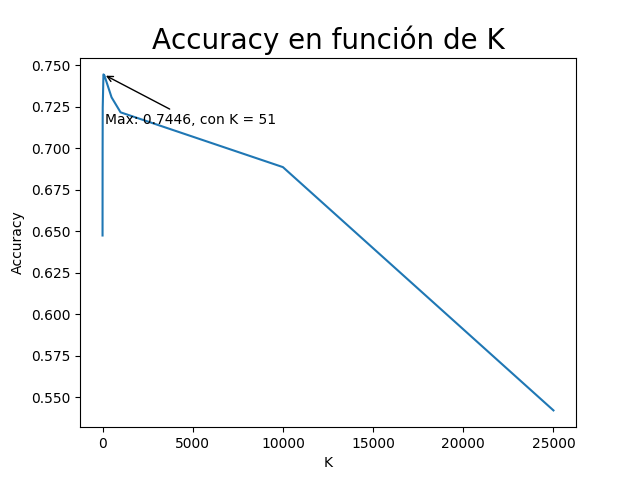
\includegraphics[ height=10cm, width=12cm]{../experimentos/graficos/graph_sin_pca_accuracy_FREQ_ORIGINAL.png}
\caption{accuracy vs. valor de\textit{ k }sin PCA con F = 0.99 y f = 0.01}
\label{fig:exp_k_orig}
\end{figure}
Con estos valores de filtrado la experimentación tardó aproximadamente 3 horas que significa un 90\% menos de tiempo que la prueba anterior.

Como podemos ver en la figura \ref{fig:exp_k_orig}, los mejores valores de\textit{ k }siguen siendo $k = 51$ y $k = 101$. El \textit{acurracy}, con estos valores de k, cambiando solo la frecuencia mínima y máxima de filtrado, varía en 0.007. Por lo tanto para las siguientes pruebas, salvo la de la sección \ref{sec:knnfrec}, vamos a filtrar el dataset con \textbf{F}$ = 0.99$ y \textbf{f}$ = 0.01$.

\subsubsection{Experimentación sobre frecuencia de palabras}
\label{sec:knnfrec}
%hipotesis
A continuación nos propusimos probar cómo varía la métrica de \textit{accuracy} al cambiar
la cantidad de palabras frecuentes y poco frecuentes que eliminamos de
nuestros \textit{Bag of Words}.
Recordamos que llamamos \textbf{f} a la frecuencia de palabras mínima a partir de la cual guardamos
palabras y \textbf{F} la frecuencia máxima a partir de la cual borramos palabras.

Suponemos que al tener una menor cantidad de palabras para cada reseña el
\textit{accuracy} al correr kNN va a ser más alto y al tener mayor cantidad de palabras va a ser peor.
Esto es debido a que las palabras más y menos frecuentes suelen meter más ruido
de lo que ayudan a clasificar.

%pruebas y gráficos
Para las pruebas, elegimos 3 valores de \textbf{f} y 3 de \textbf{F} y probamos cada valor de \textbf{f} con cada valor de \textbf{F}.
Corrimos las pruebas con $k = 51$, ya que en el experimento anterior vimos que
es un\textit{ k }razonable en cuanto a calidad de resultados.

\begin{figure}[H]
\centering
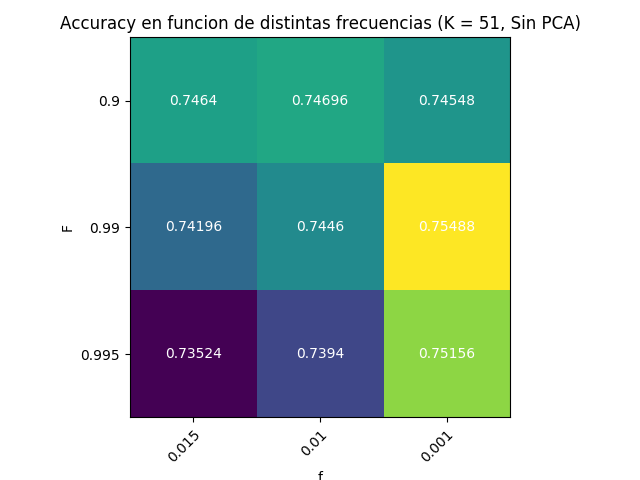
\includegraphics[ height=10cm, width=12cm]{../experimentos/graficos/graph_freq_accuracy51.png}
\caption{Accuracy vs. frecuencias con\textit{ k }= 51}
\label{fig:freq_k51}
\end{figure}

Al ver que nuestra hipótesis no se cumplió en la figura \ref{fig:freq_k51}, decidimos probar también con $k = 101$.

\begin{figure}[H]
\centering
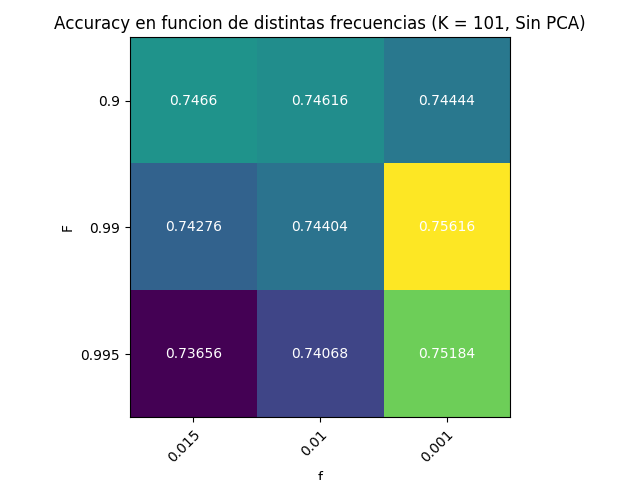
\includegraphics[ height=10cm, width=12cm]{../experimentos/graficos/graph_freq_accuracy101.png}
\caption{accuracy vs. frecuencias con\textit{ k }= 101}
\label{fig:freq_101}
\end{figure}

%conclusiones:
Tuvimos resultados parecidos para ambos\textit{ k }como se puede ver en la figura  \ref{fig:freq_k51} y \ref{fig:freq_101}, aunque ninguno concuerda con nuestra hipótesis inicial.

La combinación que menos accuracy tiene es nuestro \textbf{f} y \textbf{F} más altos, es decir,
la que elimina menos palabras de las más frecuentes (principalmente artículos
y palabras por el estilo) y muchas palabras poco frecuentes (palabras extrañas,
con \textit{typos} o en otros idiomas distintos al mayoritario, que es el inglés).

Por otro lado, la combinación que resultó en mayor \textit{accuracy}
fue cuando probamos el menor \textbf{f} y el \textbf{F} de tamaño medio.
Es decir, tenemos más \textit{accuracy} cuando borramos la menor cantidad de palabras poco
frecuentes y cuando borramos más palabras frecuentes que en el peor caso.

Esto nos dice que hay palabras que son poco frecuentes pero igualmente son
relevantes a la hora de clasificar, como pueden ser palabras que se usan en contextos
muy concretos pero con una tendencia positiva o negativa marcada.
Además, vemos que hay palabras con frecuencia alta que son relevantes, pero
hasta cierto punto. El equilibrio entre borrar pocas o muchas palabras
frecuentes parece ser cercano a $F = 0.99$.

\subsubsection{Experimentación con distintos tamaños del training dataset}
\label{sec:knnvstrain}
%hipotesis (Analizar tiempos y accuracy)

Otro experimento que nos parece interesante es cambiar el tamaño del dataset de entrenamiento.
Correremos el programa sin PCA usando el mismo dataset proporcionado por la cátedra, pero con la
diferencia que la cantidad de entradas de tipo training será un número variable y la cantidad
de entradas de tipo test serán los sobrantes. Para dividir esto, antes que nada, vamos a randomizar el dataset y
luego vamos a buscar igual cantidad de reseñas positivas que negativas para el dataset de training.

Sostenemos la hipótesis de que al aumentar el tamaño del dataset de training subirá el \textit{accuracy} de
nuestras predicciones. Pensamos esto debido a que al aplicar el algoritmo de kNN con tantos elementos
para comparar, suponemos que el vector correspondiente a una review negativa (o análogamente positiva)
tendrá muchos vecinos negativos. De la misma forma, si hay pocos elementos de training, esperamos que
una review negativa tenga pocos vecinos negativos, por lo tanto dando a lugar a vecinos positivos que
influyen en el rating.

Además, esperamos que eventualmente el crecimiento del \textit{accuracy} se estanque. Es decir, que en cierto
tamaño de dataset de training, deje de aumentar el \textit{accuracy} de las predicciones, debido a la cantidad de
vecinos de un elemento empieza a ser redundante para un \textit{k} razonable.

El siguiente gráfico muestra los resultados de correr predicciones sin PCA con diversos tamaños del training data,
con los \textit{ks} que mejores resultados dieron en experimentos anteriores. (51, 101, 501 y 1001)

%pruebas y gráficos

\begin{figure}[H]
\centering
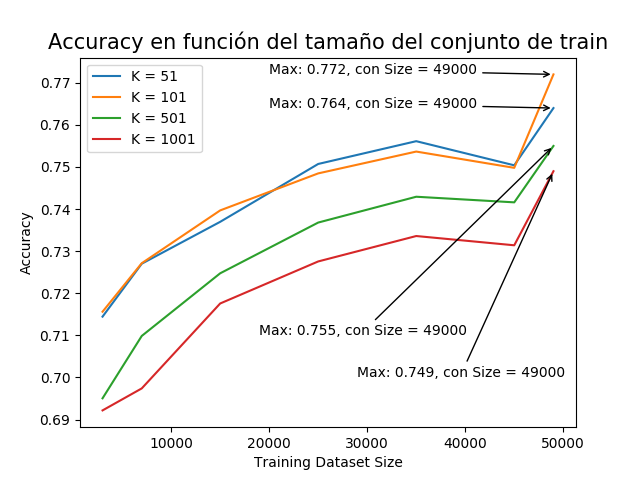
\includegraphics[ height=10cm, width=12cm]{../experimentos/graficos/graph_train_size_accuracy.png}
\caption{accuracy con distintos tamaños de training dataset}
\label{fig:exp_knn_train}
\end{figure}

Tal como esperabamos la figura \ref{fig:exp_knn_train} muestra que a medida que incrementa el tamaño del dataset de entrenamiento, también aumenta el
\textit{accuracy}. Se puede ver que cuanto mayor sea \textit{k}, los resultados de accuracy empeoran. Esto tiene sentido, dado que si hay más elementos en el algoritmo, da
lugar a nuevos vecinos para una predicción en particular que sólo son abarcables por un \textit{k} mayor.

No se puede observar que haya \textit{overfitting} al aumentar el tamaño del dataset de training, es decir, se observa que el \textit{acurracy} sigue aumentando al incrementar la cantidad de datos de entrenamiento.\\

Este experimento nos hizo pensar, que si bien aumentar el tamaño del conjunto de entrenamiento puede
mejorar las predicciones, también puede aumentar el tiempo de ejecución. Por lo tanto, planteamos un nuevo
experimento en donde ejecutamos 20 veces el algoritmo con $\textit{k} = 51$ fijo, para cinco tamaños distintos del conjunto de
entrenamiento (15000, 25000, 35000, 45000 y 49000) y luego medimos el tiempo de las predicciones
(es decir, sin tomar en cuenta el tiempo que toma cargar los datos y tokenizar).
En la figura \ref{fig:time_knn_train}, se puede ver el tiempo promedio de una \'unica predicci\'on.

\begin{figure}[H]
\centering
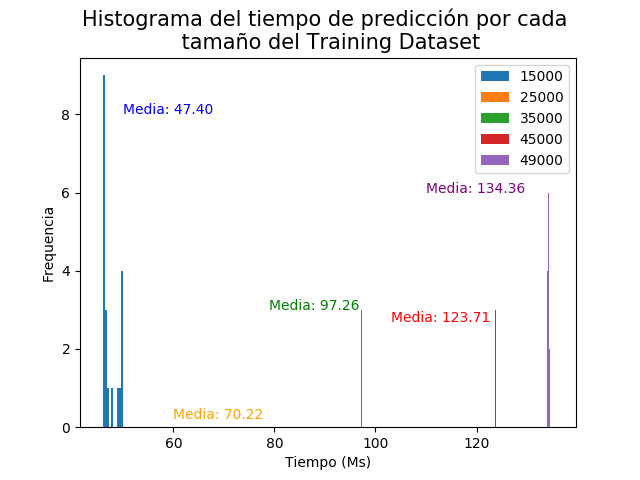
\includegraphics[ height=10cm, width=12cm]{../experimentos/graficos/graph_knn_vs_train_time.png}
\caption{tiempo de ejecución promedio de una predicción, con distintos tamaños de training dataset}
\label{fig:time_knn_train}
\end{figure}

%conclusiones:

Como era de esperar se ve que, en la figura \ref{fig:time_knn_train}, aumentar el tamaño del dataset de training implica más elementos contra quien comparar
distancias vectoriales en el algoritmo kNN, por lo tanto tiene sentido que aumente el tiempo de ejecuci\'on.
Esto es algo que tener en cuenta en la práctica, dado que se podría perder \textit{accuracy}, con tal de lograr
una predicci\'on mucho más veloz.

\subsection{Experimetación sobre PCA}

\subsubsection{Experimetación sobre tamaño del alpha}
%hipotesis
A continuación experimentamos sobre el valor de $\alpha$, siendo $\alpha$
la cantidad de componentes principales a considerar en el algoritmo de PCA.

Como hipótesis sostenemos que para los primeros valores de $\alpha$ el valor
de la métrica \textit{accuracy} va ir aumentando significativamente debido
a que las primeras componentes principales describen la mayor parte de la varianza de los datos.

Luego, a partir de determinado valor de $\alpha$ lo suficientemente grande,
conjeturamos que el valor de \textit{accuracy} comenzará a disminuir ya que
estaríamos considerando valores de la muestra de menor varianza y esto no
aportaría información sino que generaría ruido afectando la predicción de polaridad del vector.

%pruebas y gráficos
Experimentamos con distintos valores de $\alpha$, con $k = 1, 51, 101, 501, 1001, 24999$, y terminando el método de la potencia luego de 20 iteraciones.

\begin{figure}[H]
\centering
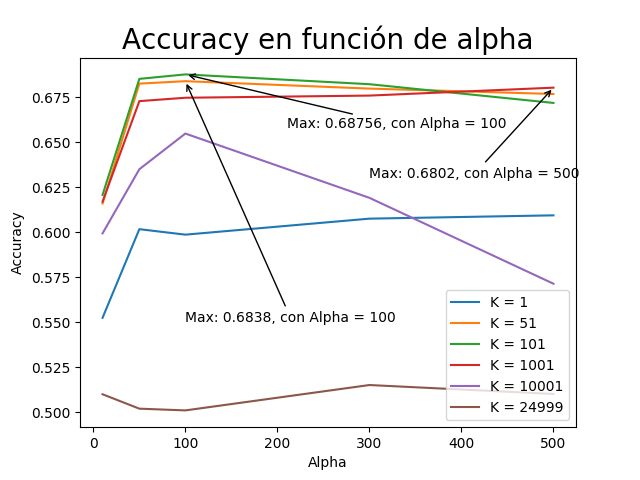
\includegraphics[ height=10cm, width=12cm]{../experimentos/graficos/graph_pca_accuracy.png}
\caption{accuracy vs. valor de alpha}
\label{fig:exp_alpha}
\end{figure}

%conclusiones:
Concluimos luego de la experimentación, viendo la figura \ref{fig:exp_alpha}, que el algoritmo de PCA es
particularmente útil para reducir la dimensionalidad de un grupo de datos.
Observamos que para valores bajos de $\alpha$ la accuracy aumenta debido a que
las primeras componentes principales describen la mayor parte de la varianza
de los datos (más, cuanto más correlacionadas estuvieran las variables originales).
Estos componentes de bajo orden a veces contienen el aspecto ``más importante''
 de la información, y las demás componentes se pueden ignorar.

\subsubsection{Experimentación sobre cantidad de iteraciones del Método de la Potencia}
%hipotesis
En esta sección mostraremos la experimentación realizada sobre distintos
valores de número de iteraciones antes de detener el Método de la Potencia
(En experimentos anteriores de PCA, este n\'umero era 20).
El mismo, como ya contamos anteriormente, es usado para calcular los autovectores
necesarios para PCA, por lo que resulta relevante detener el método en una
cantidad de iteraciones suficiente como para que el método converja, pero
no demasiado alto, ya que aumenta el tiempo de cómputo.

Nuestra hipótesis es que el \textit{accuracy} aumentará a medida que aumente
la cantidad de iteraciones, primero con una gran pendiente, pero luego de forma
más moderada hasta llegar a un techo.
Justificamos esto en que luego de cierta cantidad de iteraciones,
el método converge lo suficiente y no puede mejorar más de lo que la memoria
finita de los puntos flotantes se lo permite.

%pruebas y gráficos
A continuación, mostramos la experimentación realizada con $k = 51$ y $k = 101$,
y $\alpha = 100$ (el cual resultó ser de los mejores en el experimento anterior):

\begin{figure}[H]
\centering
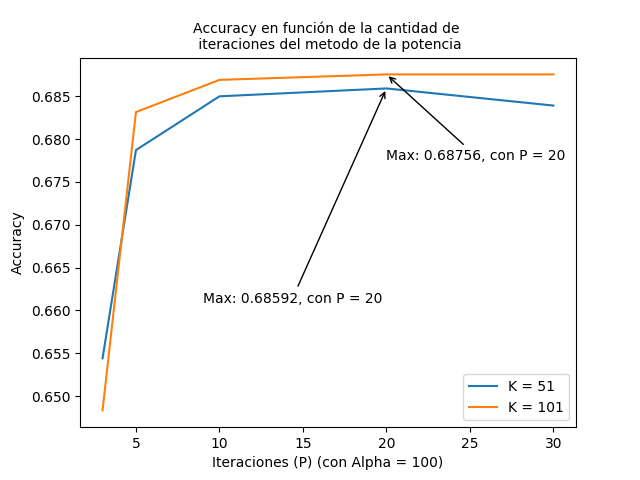
\includegraphics[ height=10cm, width=12cm]{../experimentos/graficos/graph_power_accuracy.png}
\caption{accuracy vs. cantidad de iteraciones del método de la potencia}
\label{fig:exp_met_potencia}
\end{figure}

%conclusiones:
Podemos observar que los resultados de la figura \ref{fig:exp_met_potencia} son los esperados.
En las pruebas con menor número de iteraciones se ve como el método mejora,
hasta que llega a 10 y comienza a aplanarse, sin demasiada diferencia
en la calidad de los resultados con un número de iteraciones superior.

\subsubsection{Experimentación sobre tamaño de training data}
%hipotesis (Analizar tiempos y accuracy)
Realizaremos distintas pruebas sobre el tamaño del dataset,
descripto anteriormente en la sección de Desarrollo, que utilizaremos como
Training Data para nuestro algoritmo. Este experimento es similar a uno
realizado anteriormente, pero ahora lo realizaremos con PCA.

Para este experimento, luego de randomizar el dataset proporcionado por la c\'atedra,
vamos a buscar igual cantidad de reseñas positivas que negativas para distintos tamaños
del dataset de training.

Lo que esperamos observar es, al igual que en el experimento anterior sin PCA,
que a medida que aumentemos el tamaño del Training Data, eligiendolo de igual manera que en la sección 3.1.3, el algoritmo prediga
cada vez mejor, resultando esto en un aumento en el valor de \textit{accuracy}.
Sin embargo, consideramos que este valor vaya creciendo cada vez más lento
a medida que el tamaño del Training Data es suficientemente grande,
debido a que ya no hay mucho más para ``aprender'', es decir, que la información
comienza a ser redundante y no aporta nuevo ``conocimiento'' de manera significativa.

Además, cuanto más grande sea el dataset de entrenamiento, hay que calcular
más distancias para realizar una predicción, por lo que esperamos que cada una
tome mayor tiempo.

%pruebas y gráficos
En los experimentos, utilizamos 5 tamaños distintos, que son los que vimos como más
relevantes en el experimento análogo a este sin PCA,
con $k = 51$, $k = 101$, $k = 501$ Y $k = 1001$. Al método de la potencia, lo terminamos luego de 20 iteraciones.

\begin{figure}[H]
\centering
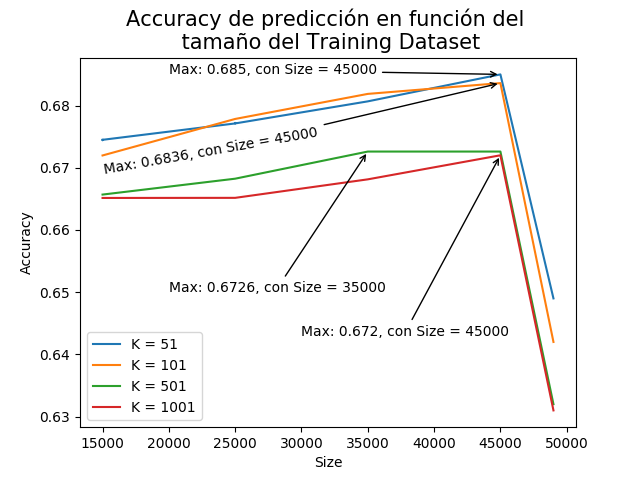
\includegraphics[ height=10cm, width=12cm]{../experimentos/graficos/graph_pca_vs_train_accuracy}
\caption{Acurracy de PCA con distintos tamaños de training dataset}
\label{fig:exp_pca_train}
\end{figure}

Para medir tiempos, ejecutamos las predicciones 20 veces, tomando el tiempo
de clasificar con kNN una vez que ya se redujeron las dimensiones con PCA.

\begin{figure}[H]
\centering
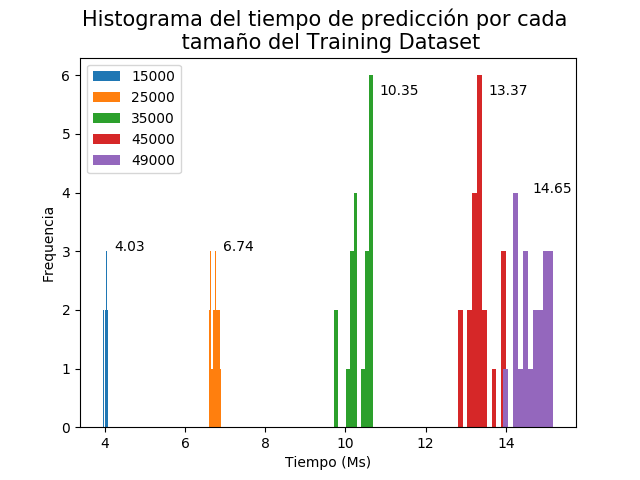
\includegraphics[ height=10cm, width=12cm]{../experimentos/graficos/graph_pca_vs_train_time.png}
\caption{tiempo de ejecución promedio de una predicción, con distintos tamaños de training dataset}
\label{fig:exp_pca_train_time}
\end{figure}

%conclusiones:
Posterior a la experimentación, viendo la figura \ref{fig:exp_pca_train}, podemos verificar nuestra hipótesis ya que el
valor de \textit{accuracy} aumenta a medida que aumentamos el tamaño del
Training Dataset, pero de forma gradual hasta que llega un punto donde el \textit{acurracy} empieza a descender. Esto nos indica que se produce \textit{overfitting}, es decir, llega un punto donde el dataset es tan grande que sobreentrenamos el sistema para poder predecir reseñas muy específicas que tienen poco relación con las reseñas que se testean.
Comparando con la Figura \ref{fig:exp_knn_train}, podemos ver que
el salto entre el \textit{accuracy} con el dataset de 15000 y el de 25000
es más pronunciado al usar kNN sin PCA que al agregarlo. Esto puede resultar de
que, al usar PCA, perdemos información que puede ser valiosa, incluyendo lo que
ganamos al aumentar el tamaño del Training Dataset.

Nuevamente, repitiendo los resultados del test sin PCA, observamos que hay un
\textit{trade-off}: con menos datos de entrenamiento,
las estimaciones resultan menos exactas, pero toman menos tiempo. De todos modos
al usar PCA el \textit{accuracy} creció relativamente poco con respecto a lo que
crecieron los tiempos de ejecución, como se ve en la figura \ref{fig:exp_pca_train_time}, por lo que es más factible usar un
dataset ``pequeño'' como el de 15000.

\subsection{Experimetación sobre kNN y PCA}
%hipotesis (Analizar tiempos y accuracy)
Para finalizar, nuestro último experimento consistirá en comparar el
tiempo de computo al ejecutar kNN con y sin PCA previo.
Nuestra hipótesis es que con PCA corra más rápido que sin, dado que disminuye
el tamaño de los vectores.

%pruebas y gráficos
Utilizamos los valores $k = 51$ y $\alpha = 100$, que en experimentos
anteriores han mostrado ser de los mejores. Computamos 18 veces los resultados,
midiendo los tiempos exclusivamente de kNN (es decir, sin contar el tiempo
de cargar los datos, tokenizar, o reducir dimensiones con PCA
en los casos que aplique).

\begin{figure}[H]
\centering
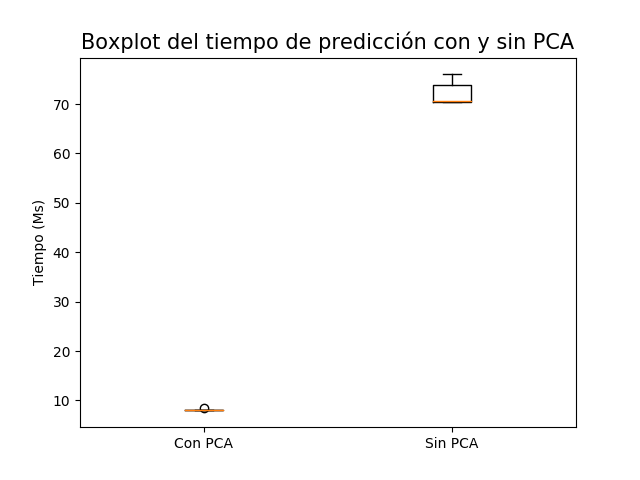
\includegraphics[ height=10cm, width=12cm]{../experimentos/graficos/graph_knn_vs_pca_time.png}
\caption{tiempo de ejecución promedio de una predicción, con y sin PCA previo}
\label{fig:exp_pca_knn}
\end{figure}

%conclusiones:
Como esperábamos, se ve en la figura \ref{fig:exp_pca_knn} que, los tiempos de ejecución bajan al ejecutar PCA antes de hacer
kNN. La contraparte es que, como se puede ver en las figuras ~\ref{fig:exp_k}
y ~\ref{fig:exp_alpha}, el \textit{accuracy} con PCA no supera el 70\%,
mientras que sin PCA llega a superar el 74\%.
La experimentación realizada nos hace pensar que, al usar PCA,
nos encontramos con un \textit{trade-off} entre velocidad y exactitud de resultados.
Esto puede resultar del hecho de que PCA descarta información
que puede resultar valiosa para la clasificación.
También es posible que la data no contenga ruido suficiente como para que
utilizar PCA mejore las métricas.
Resulta de interés realizar una experimentación más exhaustiva para comprobar que efectivamente
no existan hiperparámetros que consigan que utilizar PCA aumente el \textit{accuracy},
aunque queda fuera del alcance del presente trabajo.
% Esto nos muestra que, al usar
% PCA, nos encontramos con un \textit{trade-off} entre velocidad y exactitud
% de resultados. Esto puede resultar del hecho de que PCA descarta información
% que puede resultar valiosa para la clasificación.
